\documentclass[journal]{IEEEtran}
\IEEEoverridecommandlockouts

% ==========================================================
% PACKAGES
% ==========================================================

% *** CITATION PACKAGES ***
\usepackage[style=ieee]{biblatex}
\bibliography{example_bib.bib}

% *** MATH PACKAGES ***
\usepackage{amsmath}

% *** PDF, URL AND HYPERLINK PACKAGES ***
\usepackage{url}
\usepackage{graphicx}
\usepackage{float}

\hyphenation{op-tical net-works semi-conduc-tor}

% Desactiva la marca numérica automática de las notas al pie
\makeatletter
\renewcommand{\@makefnmark}{}
\makeatother

% ==========================================================
% DOCUMENT
% ==========================================================

\begin{document}

% ==========================================================
% TITLE
% ==========================================================

\title{
Beyond Fraud Detection: Uncovering Anomalous Financial Behavior Through Unsupervised Learning
\\[9pt]
\small{Beyond the Transaction: An Unsupervised Approach to Financial Anomaly Detection}
}

% ==========================================================
% AUTHORS
% ==========================================================

\author{
    \IEEEauthorblockN{
        J. A. Melchor Soto,
        R. Fortanell Canedo,
        E. C. Huerta, and
        I. Téllez Antillón\\
    }
    \IEEEauthorblockA{
        \textit{ITESO, Universidad Jesuita de Guadalajara}
        Jalisco, México\\
    \IEEEauthorblockB{
            jose.melchor@iteso.mx,
            rolando.fortanell@iteso.mx,
            emiliano.contreras@iteso.mx,
            ismael.tellez@iteso.mx
        }
    }
}

% ==========================================================
% RUNNING HEAD
% ==========================================================

\markboth{
BEYOND FRAUD DETECTION, SEPTEMBER 2026
}{
Melchor Soto \MakeLowercase{\textit{et al.}}: Beyond Fraud Detection
}

\maketitle

% ==========================================================
% ABSTRACT
% ==========================================================

\begin{abstract}
Detecting financial fraud is usually a supervised learning problem, but in practice, labeled examples of fraud are rarely available. This study takes a different approach: instead of trying to classify transactions as fraudulent or not, it looks for transactions that simply behave differently from the rest. Using an Isolation Forest model trained on 3,293 unlabeled US bank transactions with a strictly temporal split, unusual transactions are flagged and then explored from several angles, including how they change over time, what makes them behave differently, and where they tend to occur geographically. To make sure these findings are not just noise, the model is refit under ten random seeds and SHAP is used to understand which features drive each anomaly. An interactive map of the United States is also used to show where the anomalies are concentrated. The anomaly ranking proved stable across seeds (mean Spearman $\rho = 0.899$), whereas the binary flag was less so (mean Jaccard $= 0.689$); 16 test transactions were flagged in every run. A threshold fixed on training data (2\% contamination) flagged 2.32\% of validation and 6.79\% of test transactions, revealing a progressive score drift that begins months before the test window. Flagged transactions differ from normal ones mainly through amount relative to its context, while the model's overall notion of anomaly is multifactorial. Finally, the geographic pattern is shown to be driven by sample size and by the synthetic rows added to give the map full coverage, so it must be read descriptively. All of this is obtained without ever needing labeled fraud data.
\end{abstract}

\begin{IEEEkeywords}
anomaly detection, unsupervised learning, fraud detection, Isolation Forest, financial data, model stability, SHAP, temporal drift
\end{IEEEkeywords}

% ==========================================================
% 1. INTRODUCTION
% ==========================================================


\section{Introduction}

\IEEEPARstart{F}{inancial} fraud represents a significant challenge for financial institutions, as large volumes of transactions must be continuously analyzed to identify unusual behavior. Most financial transactions correspond to legitimate activity, while only a small portion may exhibit patterns that require further investigation. Consequently, identifying potentially anomalous transactions within a large amount of normal financial activity is difficult to perform manually and requires automated detection mechanisms.

A common approach to financial fraud detection is to formulate the problem as a supervised classification task, where historical transactions are assigned labels such as fraudulent or legitimate. However, obtaining reliable fraud labels can be difficult, incomplete, or unavailable in real-world financial datasets. In addition, fraudulent behavior may change over time, making previously observed patterns insufficient to describe new forms of anomalous activity. These limitations reduce the applicability of approaches that depend entirely on previously labeled fraudulent transactions.

Anomaly detection provides an alternative perspective for addressing this problem. Instead of learning predefined fraud classes, anomaly detection methods aim to identify observations that deviate from the general behavior present in the data. This formulation is particularly relevant when anomalous cases are rare and reliable labels are not available, allowing unusual transactions to be identified without requiring previously confirmed fraud cases. Similar approaches have been explored in other domains where anomalous behavior cannot be completely specified in advance, motivating the use of unsupervised methods for detecting deviations from normal patterns \cite{chandola2009anomaly}.

Several machine learning techniques have been proposed for anomaly detection, including statistical methods, clustering, dimensionality reduction, and tree-based approaches. Among these techniques, Isolation Forest provides an unsupervised approach that identifies observations that can be isolated more easily than the majority of the data. This makes it suitable for analyzing high-dimensional transaction data in which anomalous observations may not follow a previously known pattern \cite{liu2008isolation}.

However, identifying anomalous transactions is only one part of the problem. An anomaly score by itself does not explain whether the detected observation represents a meaningful behavioral deviation, how consistently it is identified, or how anomalous behavior is distributed across different dimensions of the data. Therefore, a more complete analysis should consider not only the detection of anomalies but also their temporal, behavioral, and geographic characteristics. In addition, evaluating the stability of detected anomalies across different model configurations can provide information about the robustness of the resulting observations.

In this work, we reformulate financial fraud detection as an unsupervised anomaly detection problem in the absence of confirmed fraud labels. We apply an Isolation Forest model to identify transactions that deviate from the observed behavioral patterns and subsequently analyze the detected anomalies from multiple perspectives. The analysis considers their temporal distribution, behavioral characteristics, feature contributions, geographic distribution, and stability across multiple model runs. Rather than treating detected anomalies as confirmed fraudulent transactions, the proposed approach uses them as observations that require further analysis and investigation.

The main contribution of this work is therefore not limited to detecting anomalous transactions but to providing a multidimensional characterization of unusual financial behavior. By combining unsupervised detection with robustness analysis, interpretability, and geographic visualization, this study provides a framework for investigating anomalous financial activity when reliable fraud labels are not available. Concretely, the contributions are:
\begin{itemize}
    \item a leakage-free, temporally split unsupervised pipeline whose every output is an anomaly score rather than a fraud probability;
    \item a stability protocol that separates the consistency of the anomaly \emph{ranking} from that of the binary \emph{flag}, and isolates a core of transactions flagged under every seed;
    \item evidence that a train-derived threshold does not keep its contamination rate over time, together with a month-by-month view of when the drift begins;
    \item a behavioral and SHAP-based characterization of what distinguishes flagged transactions, and
    \item an interactive map of the United States, together with an explicit audit of how sample size and synthetic coverage rows shape the geographic pattern it displays.
\end{itemize}

% ==========================================================
% 1b. HYPOTHESES  (new section, from the hypothesis document)
% ==========================================================

\section{Hypotheses}

The general hypothesis of this work is that, even without fraud labels, an unsupervised model can identify unusual transactions in a way that is \emph{useful and characterizable}: its ranking will be consistent, the behavior of the transactions it flags will be distinguishable from that of normal transactions, and its limitations, particularly over time and across geography, will be identifiable and measurable.

Five specific hypotheses follow from it. Each is stated together with the observable evidence used to assess it in Section~\ref{sec:hypothesis_eval}.

\textbf{H1 (stability).} The ranking of transactions by anomaly score will be stable across random seeds, whereas the binary decision of flagging a transaction will be less stable, because the variation concentrates on the transactions closest to the threshold. \emph{Evidence:} pairwise Spearman correlation of scores higher than pairwise Jaccard similarity of flagged sets, and a bimodal per-transaction stability.

\textbf{H2 (temporal transfer).} A fixed threshold, computed only from training data, will not preserve the expected anomaly rate in later periods, because of a shift in the distribution of the scores. \emph{Evidence:} validation and test flagged rates compared with the 2\% target, across all seeds and within the real (non-synthetic) rows alone.

\textbf{H3 (behavioral signature).} Flagged transactions will differ from normal ones mainly through amount-related variables, both in absolute terms and relative to their context (hour, state, merchant, and account). \emph{Evidence:} standardized mean gaps between flagged and normal transactions.

\textbf{H4 (multifactorial anomaly).} The model's notion of anomaly will be multifactorial, with no single variable dominating the score. \emph{Evidence:} spread of mean absolute SHAP values across feature categories.

\textbf{H5 (descriptive geography).} The observed geographic patterns will be descriptive and will depend on each state's sample size, so they cannot be interpreted as evidence of a higher real fraud risk. \emph{Evidence:} relation between state support and anomaly rate, and comparison between states covered by real and by synthetic rows.

% ==========================================================
% 2. TERMINOLOGY AND PROBLEM DEFINITION
% ==========================================================

\section{Background}

\subsection{Preliminary Definitions}

\textit{Fraud detection} is the task of deciding whether a transaction is fraudulent; it requires a ground-truth label against which a decision can be checked. \textit{Anomaly detection} is the task of finding observations that deviate markedly from the behavior of most of the data \cite{chandola2009anomaly}; it does not require a label. In this work, an \textit{anomaly score} $s(x)\in[0,1]$ measures how unusual a transaction $x$ is with respect to the distribution observed during training, where a larger value indicates a more unusual transaction. A transaction is \textit{flagged as anomalous} when its score is at or above the \textit{operating threshold} $\tau$, and the \textit{contamination} $c$ is the expected proportion of anomalies in the data, fixed at $c=0.02$. Learning is \textit{unsupervised}: the model is fitted on transactions alone, without any target variable.

It is important to distinguish an anomalous transaction from a confirmed fraudulent one. Because the dataset contains no fraud label, the score is not a probability of fraud and the number of flagged transactions is not a fraud count. Throughout the paper, flagged transactions are therefore described as \emph{unusual relative to the training distribution}, and never as detected fraud.

\subsection{Challenges}

The first challenge is the \textit{absence of ground truth}: without labels it is impossible to compute supervised metrics such as precision, recall, or AUC, and the quality of the model must be assessed indirectly through its stability, its interpretability, and its coherence with basic intuition. The second is \textit{class imbalance}: anomalies are, by construction, a small minority (2\% here), so any estimate computed on them rests on few observations. The third is \textit{non-stationarity}: transactional behavior changes over time, so a threshold calibrated on historical data may not transfer to later periods. The fourth is the \textit{sensitivity of binary decisions near the threshold}, where small variations of the model change which transactions are flagged even when the ranking is consistent. Finally, \textit{interpretability} is harder than in the supervised case, because there is no label to which feature contributions can be anchored, and the dataset is small compared with those typically used in fraud analytics, which limits the precision of any estimate, especially per state or over short windows.

% ==========================================================
% 3. RELATED WORK
% ==========================================================

\section{Related Work}

Most of the work on transactional fraud detection is supervised. Because fraud is a very small fraction of the total, conventional classifiers tend to ignore the minority class, and accuracy can remain high even when no fraud is detected. Chawla et al. \cite{chawla2002smote} proposed SMOTE, an oversampling technique that generates synthetic examples of the minority class, and more recent work has explored cost-sensitive learning, where the decision threshold is chosen to minimize the monetary cost of errors \cite{danang2025cost}. Graph neural networks that model accounts, merchants, and devices as connected nodes have also been proposed, which makes it possible to capture coordinated fraud \cite{cheng2024gnn}. All of these approaches, however, depend on a reliable set of labeled fraud cases.

When no labels are available, anomaly detection offers an alternative; a broad review of the field is presented in \cite{chandola2009anomaly}. Isolation Forest \cite{liu2008isolation} differs from density- or distance-based methods: instead of modeling normal behavior, it explicitly isolates observations through random partitions, so that anomalies, being few and different, require fewer cuts. Its efficiency and suitability for high-dimensional tabular data make it a common baseline. To explain why an observation was flagged, SHAP \cite{lundberg2017unified} attributes the model output to its features through Shapley values, and its tree algorithm \cite{lundberg2020trees} computes these attributions efficiently.

This work sits between these lines. Rather than proposing a new detector, it applies a standard unsupervised model and focuses on what can be said about its output without labels: how stable it is, how its threshold behaves over time, which variables drive it, and how flagged transactions are distributed across states. The research gap it addresses is precisely this evaluation layer, which is usually replaced by supervised metrics that are unavailable in the unlabeled setting.

% ==========================================================
% 4. DATASET AND EXPERIMENTAL SETUP
% ==========================================================

\section{Dataset and Experimental Setup}

\subsection{Dataset}

The source data is the public \textit{Bank Transaction Dataset for Fraud Detection}, which contains 2,512 US bank transactions from 495 accounts. Despite its name, it is distributed \emph{without a fraud label}, so it is an anomaly detection dataset and not a classification one. Each record includes the transaction amount, type (debit or credit), channel (ATM, branch, or online), timestamp, city, merchant and device identifiers, customer age and occupation, session duration, login attempts, and account balance.

The working dataset used in every experiment has 3,293 transactions from 654 accounts, distributed across 52 US states and territories, covering 2 January 2023 to 1 January 2024. Because it lacks a fraud label, every model output is an anomaly score and never a fraud probability or a count of confirmed fraud. Across the full period, the average transaction amount is \$298.13 and the average account balance is \$5,145.78.

\subsection{Synthetic Geographic Coverage and Its Purpose}
\label{sec:augmentation}

One objective of the study is to present the anomalies on an interactive map of the United States. The 43 city names in the source data, however, resolve to only 27 of the 52 polygons in the GeoJSON file that defines the map, so 25 states would appear empty. To give every polygon a value, 781 synthetic rows were added for those 25 states (Fig.~\ref{fig:dataset_map}). For each uncovered state, a representative city was assigned and $n=\mathrm{clip}(\mathrm{round}(10\cdot P),20,100)$ rows were created, where $P$ is the state population in millions. Rows were drawn by resampling the \emph{whole} real dataset with replacement; only the location and the transaction and account identifiers were replaced, the amount, balance, and duration received a multiplicative jitter $\times\exp(\mathcal{N}(0,0.15))$ clipped to the real range, and the timestamp was shifted by $\mathcal{U}(-3,3)$ days within the real span. Real rows are copied unchanged, and synthetic rows remain identifiable by their identifier prefix.

The purpose of these rows is exclusively \emph{visual coverage}: they are statistically faithful to the national distribution but not to any real local behavior. Section~\ref{sec:res_synthetic} shows that they nonetheless influence the model, which is why every geographic result is accompanied by the real/synthetic distinction.

\begin{figure}[!t]
\centering
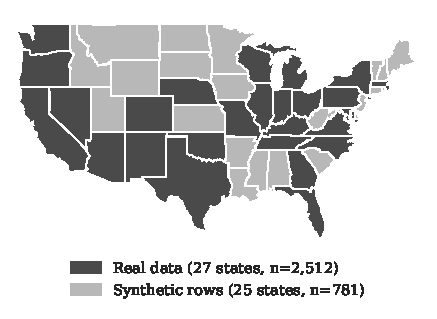
\includegraphics[width=\columnwidth]{figures/fig02_dataset_map.pdf}
\caption{Composition of the working dataset by state. Dark: states covered by the 2,512 real transactions. Light: the 25 states covered only by the 781 synthetic rows added so that the US map has a value for every polygon (Alaska, Hawaii, and Puerto Rico, both synthetic, are not drawn).}
\label{fig:dataset_map}
\end{figure}

\subsection{Feature Engineering}

From the original fields, 85 features covering temporal, behavioral, geographic, and demographic aspects were built. \textit{Temporal} features include the month, the hour, and indicators of night-time and weekend transactions. \textit{Transaction-level} amount features include the raw amount and its logarithm, the logarithm of the account balance, and the ratio between amount and balance. \textit{Contextual deviation} features express how far the amount of a transaction departs from what is usual for its hour, state, merchant, or account (e.g., \texttt{Amount\_Dev\_Hour} and \texttt{Amount\_Dev\_Account}). \textit{Account-level} activity is represented by the number of transactions per account and the login attempts. Categorical fields such as state, transaction type, channel, and customer occupation are one-hot encoded, and the frequency of each state in the data is added as a \textit{geographic} feature. All statistics used by these features are fitted on the training window only and then applied to the later windows.

\subsection{Temporal Data Split}

The data were split temporally and not at random: the model is trained on the past, the threshold is checked on a recent period, and evaluation is performed once on the future. A random split would leak future behavior into training and overestimate the generalization capacity. Table~\ref{tab:split} summarizes the three windows.

\begin{table}[!t]
\renewcommand{\arraystretch}{1.2}
\caption{Temporal Split of the Data}
\label{tab:split}
\centering
\begin{tabular}{lrcc}
\hline
\textbf{Window} & \textbf{$n$} & \textbf{Start} & \textbf{End} \\
\hline
Training   & 2,431 & 2023-01-02 & 2023-10-03 \\
Validation &   302 & 2023-10-04 & 2023-11-02 \\
Test       &   560 & 2023-11-03 & 2024-01-01 \\
\hline
\end{tabular}
\end{table}

% ==========================================================
% 5. METHODOLOGY
% ==========================================================

\section{Methodology}

Fig.~\ref{fig:pipeline} summarizes the full pipeline: the detection stage on top and the five analyses applied to its output below.

\begin{figure*}[!t]
\centering
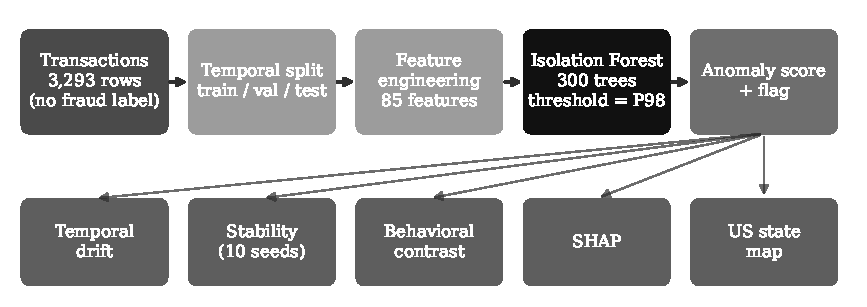
\includegraphics[width=0.9\textwidth]{figures/fig01_pipeline.pdf}
\caption{Overview of the methodology. The unlabeled transactions are split in time, transformed into 85 features, and scored by an Isolation Forest whose threshold is fixed at the 98th percentile of training scores. The resulting scores and flags are then analyzed from five angles.}
\label{fig:pipeline}
\end{figure*}

\subsection{Isolation Forest}

Isolation Forest \cite{liu2008isolation} builds an ensemble of random trees that partition the data recursively by choosing a feature and a split value at random. Observations far from the majority are isolated with fewer cuts, so their average path length $E(h(x))$ is shorter. The model was selected because it does not require labels, scales well to high-dimensional tabular data, and does not assume any specific form of anomalous behavior. The main model uses 300 trees, an expected contamination of 0.02, and a random seed of 42. The configuration was fixed before the analysis and was not tuned in response to any subsequent result.

\subsection{Anomaly Score and Threshold}

The path length is converted into the classic anomaly score
\begin{equation}
    s(x,n) = 2^{-\frac{E(h(x))}{c(n)}},
    \label{equation:anomaly_score}
\end{equation}
where $c(n)$ is the average path length of an unsuccessful search in a binary tree built on $n$ points. In the pipeline, this score is rescaled to $[0,1]$ so that higher always means more unusual. The operating threshold is
\begin{equation}
    \tau = Q_{1-c}\big(\{s(x): x \in \mathcal{D}_{\text{train}}\}\big) = 0.710495,
    \label{equation:threshold}
\end{equation}
i.e., the 98th percentile of the training scores, which corresponds to the 2\% contamination target. It is fixed using the training window only and applied unchanged to validation and test. It is thus a \emph{policy decision} and not a value learned against labels.

\subsection{Stability Analysis}

To measure how reliable the flagged transactions are, the same configuration was refit ten times with different seeds (42 to 51), each with its own train-derived threshold, and evaluated on the same 560-transaction test window. Two complementary measures were computed over the 45 pairs of runs. The Jaccard similarity between flagged sets $F_i$ and $F_j$,
\begin{equation}
    J(F_i,F_j)=\frac{|F_i\cap F_j|}{|F_i\cup F_j|},
\end{equation}
reflects agreement on the binary decision, while the Spearman correlation between the score vectors is threshold-independent and reflects agreement on the ranking. In addition, the stability of each transaction was defined as the fraction of the ten runs in which it was flagged. Since most transactions are never flagged, it is also reported conditional on having been flagged at least once.

\subsection{Behavioral and Geographic Analysis}

Flagged and normal test transactions were compared feature by feature through the standardized difference between their means. Feature importance was computed with SHAP \cite{lundberg2017unified} using its tree explainer \cite{lundberg2020trees} on a sample of 560 transactions, as the mean absolute SHAP value of each feature. As an additional check, and not as validation, the model was compared with a transparent hand-built rule based on high amount, login attempts, unusual hour, and extreme session duration.

Geographically, the anomaly rate per state was computed on the full scored dataset, requiring a minimum support of 15 transactions, and state names were reconciled with the GeoJSON file so that all 52 states could be drawn. Every state-level result is further split into states covered by real and by synthetic rows. Hour and day-of-week rates use a minimum support of 20 transactions per bucket.

\subsection{Interactive Geographic Visualization}

The results are served by a REST API and displayed in a web dashboard. Its central element is an interactive choropleth of the United States in which each state is colored by its anomaly rate; clicking or searching a state opens a card with its number of transactions, flagged transactions, rate, and mean anomaly score, and states below the support floor are marked. The dashboard also shows the score distribution and the anomaly rate by hour, day, channel, and transaction type. The static maps in this paper (Figs.~\ref{fig:dataset_map} and~\ref{fig:state_map}) are drawn from the same GeoJSON and the same artifacts as the interactive map.

% ==========================================================
% 6. RESULTS
% ==========================================================

\section{Results}

\subsection{Anomaly Detection Results}

Table~\ref{tab:split_metrics} reports the score statistics per window. By construction, 2.02\% of training transactions are flagged (49 of 2,431). The rate stays close to the target on validation (2.32\%, 7 of 302) but rises to 6.79\% on test (38 of 560). Fig.~\ref{fig:score_threshold} shows why: the test distribution has a heavier right tail than the training one, with a 99th percentile of 0.957 versus 0.776, and a visible cluster of transactions with scores above 0.9 that is almost absent during training.

\begin{table}[!t]
\renewcommand{\arraystretch}{1.2}
\caption{Anomaly Score Statistics per Window ($\tau = 0.710$)}
\label{tab:split_metrics}
\centering
\begin{tabular}{lrrrrrr}
\hline
\textbf{Window} & \textbf{$n$} & \textbf{Flag.} & \textbf{Rate} & \textbf{Mean} & \textbf{P95} & \textbf{P99} \\
\hline
Train      & 2,431 & 49 & 2.02\% & 0.361 & 0.625 & 0.776 \\
Validation &   302 &  7 & 2.32\% & 0.424 & 0.639 & 0.855 \\
Test       &   560 & 38 & 6.79\% & 0.423 & 0.746 & 0.957 \\
\hline
\end{tabular}
\end{table}

\begin{figure}[!t]
\centering
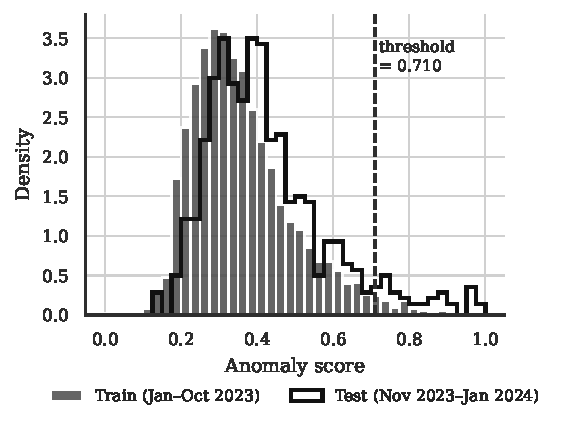
\includegraphics[width=\columnwidth]{figures/fig03_score_threshold.pdf}
\caption{Anomaly score distribution of the training (filled) and test (outline) windows, normalized to equal area. The dashed line is the operating threshold fixed on training data. The test tail beyond the threshold is clearly heavier.}
\label{fig:score_threshold}
\end{figure}

When the entire dataset is scored with the final model, which is the view used by the map and the dashboard, 108 transactions (3.28\%) are flagged. They account for \$93,262.77, that is, 9.5\% of the \$981,758.06 transacted, so flagged transactions concentrate roughly three times their share of value.\footnote{In the full-dataset view, account-level features are recomputed over all rows, so the per-window counts (58/10/40) differ slightly from the protocol counts (49/7/38) of Table~\ref{tab:split_metrics}. All protocol metrics use the latter.}

\subsection{Temporal Distribution Shift}

The test rate is 3.4 times both the contamination target and the training rate, even though the model and the threshold are unchanged (Fig.~\ref{fig:split_rates}). This shift is not an artifact of seed 42: when the model is refit with seeds 42--51, each with its own training threshold, the test rate ranges from 4.64\% to 6.79\% (mean 5.54\%), always well above 2\%.

\begin{figure}[!t]
\centering
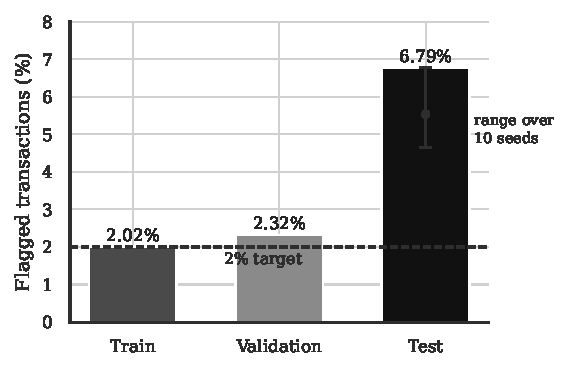
\includegraphics[width=\columnwidth]{figures/fig04_split_rates.pdf}
\caption{Share of flagged transactions per window for the main model. The dashed line is the 2\% contamination target; the error bar on the test bar spans the rates obtained with the ten seeds.}
\label{fig:split_rates}
\end{figure}

Breaking the rate down by month shows that the drift is gradual rather than abrupt (Fig.~\ref{fig:monthly}). From January to July 2023, the monthly flagged rate stays between 1.7\% and 1.9\%; it then increases to 3.2\% in August and 5.3\% in September, both still inside the training window, and reaches 6.8\% in November and 7.5\% in December. The mean score follows the same pattern (0.35--0.37 from January to July versus 0.42--0.44 from October to December). Validation, with a 2.32\% rate, sits on the transition. The shift therefore starts before the test window and accumulates over time; a cutoff estimated on January--October data averages over months with very different score levels.

\begin{figure}[!t]
\centering
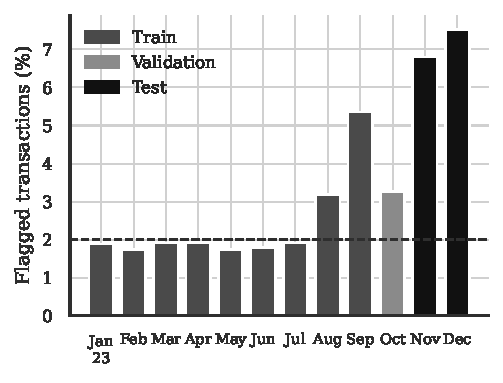
\includegraphics[width=\columnwidth]{figures/fig05_monthly_drift.pdf}
\caption{Monthly share of flagged transactions with the final model, colored by window (months with fewer than 20 transactions omitted). The rate is flat until July and rises steadily from August onward.}
\label{fig:monthly}
\end{figure}

\subsection{Effect of the Synthetic Coverage Rows}
\label{sec:res_synthetic}

Although the synthetic rows were added only for map coverage, the model flags them far more often than real rows: 7.30\% (57 of 781) versus 2.03\% (51 of 2,512) on the full dataset. Fig.~\ref{fig:real_synth} shows that this gap appears in every window, which is consistent with the jitter and the small, newly created account pools producing combinations that are rare in training and therefore easy to isolate.

Crucially, the temporal shift persists when only real transactions are considered: their flagged rate grows from 1.5\% in training to 2.3\% in validation and 4.2\% in test, a 2.8-fold increase. The synthetic rows amplify the drift (5.3\% to 16.5\%) but do not create it.

\begin{figure}[!t]
\centering
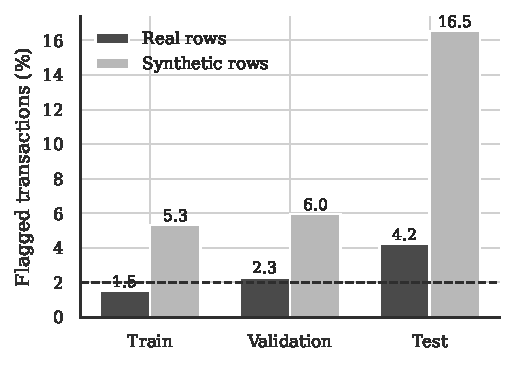
\includegraphics[width=\columnwidth]{figures/fig06_real_vs_synthetic.pdf}
\caption{Share of flagged transactions per window for real and synthetic rows. Synthetic rows are flagged more often in every window, but the rise from training to test is also present in real rows alone.}
\label{fig:real_synth}
\end{figure}

\subsection{Stability and Robustness}

Across the 45 seed pairs, the mean Jaccard similarity of the flagged sets is 0.689 (median 0.686, s.d. 0.065, range 0.568--0.862), while the mean Spearman correlation of the scores is 0.899 (median 0.901, s.d. 0.014, range 0.869--0.926). The two distributions do not overlap (Fig.~\ref{fig:stability}a): the model agrees much more on \emph{how unusual} each transaction is than on \emph{which} transactions cross a hard cutoff, and its ranking is also less sensitive to the seed, as the standard deviation of $\rho$ is almost five times smaller.

Of the 560 test transactions, 508 (90.7\%) are never flagged and 52 (9.3\%) are flagged at least once. Among these 52, the stability distribution is bimodal (Fig.~\ref{fig:stability}b): 21 are borderline cases flagged in one to four runs, while 26 are flagged in at least eight runs and \textbf{16 (2.86\% of the test window) are flagged in all ten runs}. The median conditional stability is 0.75 (mean 0.596). Table~\ref{tab:stability} summarizes these cut-offs. The 16 transactions flagged in every run form the most defensible anomaly set produced by the model; Fig.~\ref{fig:score_vs_stab} in the Appendix shows that they all have mean scores above 0.80, whereas the borderline cases spread between 0.58 and 0.84, i.e., around the per-seed thresholds (0.67--0.78).

\begin{figure*}[!t]
\centering
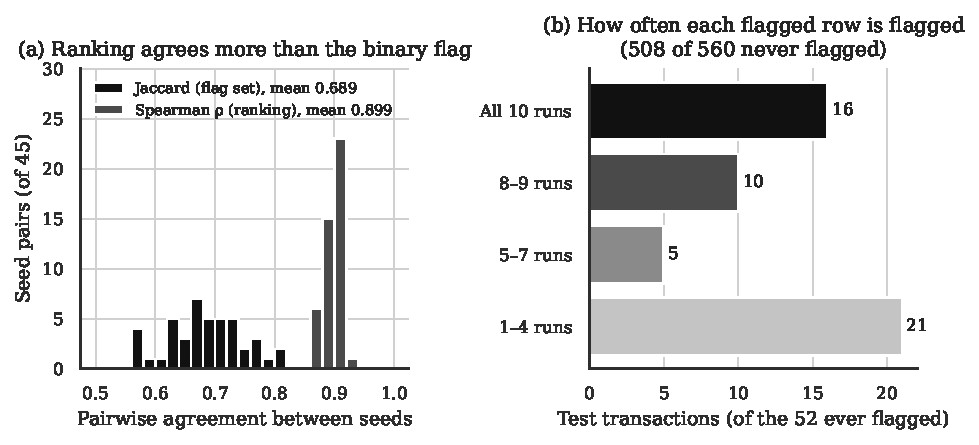
\includegraphics[width=0.85\textwidth]{figures/fig07_stability.pdf}
\caption{Stability across ten seeds. (a) Distribution of pairwise agreement over the 45 seed pairs: Jaccard similarity of flagged sets versus Spearman correlation of scores. (b) Number of runs in which each of the 52 ever-flagged test transactions is flagged; 16 are flagged in every run.}
\label{fig:stability}
\end{figure*}

\begin{table}[!t]
\renewcommand{\arraystretch}{1.2}
\caption{Per-Transaction Stability on the Test Window ($n=560$)}
\label{tab:stability}
\centering
\begin{tabular}{lrr}
\hline
\textbf{Flagged in} & \textbf{Transactions} & \textbf{\% of test} \\
\hline
All 10 runs ($=100\%$)  & 16 & 2.86\% \\
$\geq 8$ runs ($\geq 80\%$) & 26 & 4.64\% \\
$\geq 5$ runs ($\geq 50\%$) & 31 & 5.54\% \\
$\geq 1$ run ($> 0\%$)      & 52 & 9.29\% \\
\hline
\end{tabular}
\end{table}

\subsection{Behavioral Patterns}

Table~\ref{tab:contrast} and Fig.~\ref{fig:contrast} compare flagged and normal transactions in the test window. The five largest standardized gaps all concern the amount: flagged transactions average \$877.60 versus \$272.98 for normal ones (gap 1.94), and they are also large \emph{relative to their context}, i.e., to their hour (1.93), state (1.92), and merchant (1.87), and relative to the account balance (1.83). The deviation from the account's own history (0.99) is smaller but still positive. The largest non-amount gap is the weekend indicator (34\% of flagged transactions versus 4\% of normal ones), followed by occupation \textit{Student}, night-time, and login attempts (1.45 versus 1.07 on average). Flagged transactions also occur earlier in the day (12.6 h versus 15.6 h on average) and on accounts with lower balances.

\begin{table}[!t]
\renewcommand{\arraystretch}{1.2}
\caption{Largest Standardized Gaps, Flagged vs. Normal (Test)}
\label{tab:contrast}
\centering
\begin{tabular}{lrrr}
\hline
\textbf{Feature} & \textbf{Flagged} & \textbf{Normal} & \textbf{Gap} \\
\hline
TransactionAmount       & 877.60 & 272.98 & 1.94 \\
Amount\_Dev\_Hour       & 2.180 & $-0.067$ & 1.93 \\
Amount\_Dev\_USState    & 2.124 & $-0.075$ & 1.92 \\
Amount\_Dev\_MerchantID & 2.717 & $-0.051$ & 1.87 \\
Amount\_To\_Balance\_Ratio & 1.264 & 0.127 & 1.83 \\
Is\_Weekend             & 0.342 & 0.038 & 1.29 \\
Log\_Transaction\_Amount & 6.351 & 5.073 & 1.00 \\
Amount\_Dev\_Account    & 4.941 & 0.592 & 0.99 \\
\hline
\end{tabular}
\end{table}

\begin{figure}[!t]
\centering
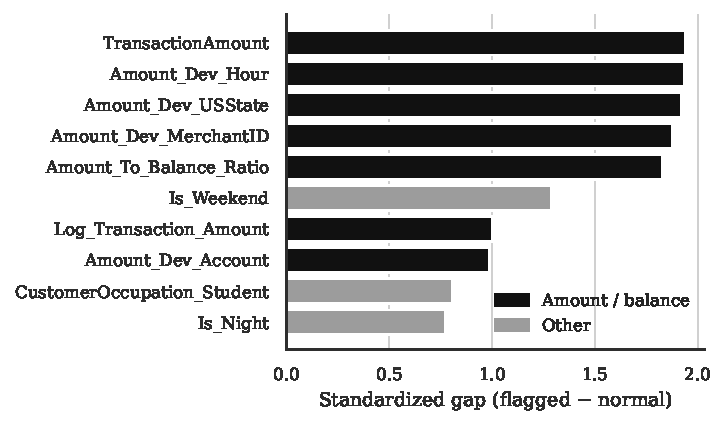
\includegraphics[width=\columnwidth]{figures/fig08_feature_contrast.pdf}
\caption{Top ten standardized gaps between flagged and normal test transactions. Dark bars are amount or balance features.}
\label{fig:contrast}
\end{figure}

\subsection{Temporal Activity Patterns}

Over the full dataset, the anomaly rate depends strongly on when a transaction occurs (Fig.~\ref{fig:temporal}). Transactions between 00:00 and 04:59 are flagged at 19.2\% (29 of 151), against 2.4\% between 06:00 and 23:59. Weekend transactions are flagged at 16.9\% on Saturday (20 of 118) and 18.8\% on Sunday (18 of 96), while every weekday stays between 1.5\% and 3.2\%. Both slots are \emph{rare} in the data: transactions between 00:00 and 04:59 and weekend transactions represent only 4.6\% and 6.5\% of all records, respectively. This is consistent with how Isolation Forest works, since rare values are isolated with few cuts, and should be read as rarity rather than as risk. By category, credit transactions are flagged more often than debit ones (6.0\% vs. 2.5\%), and students more often than the other occupations (5.9\% vs. 2.3--2.4\%); by channel, the rate is 3.8\% at branches, 3.7\% online, and 2.3\% at ATMs.

\begin{figure*}[!t]
\centering
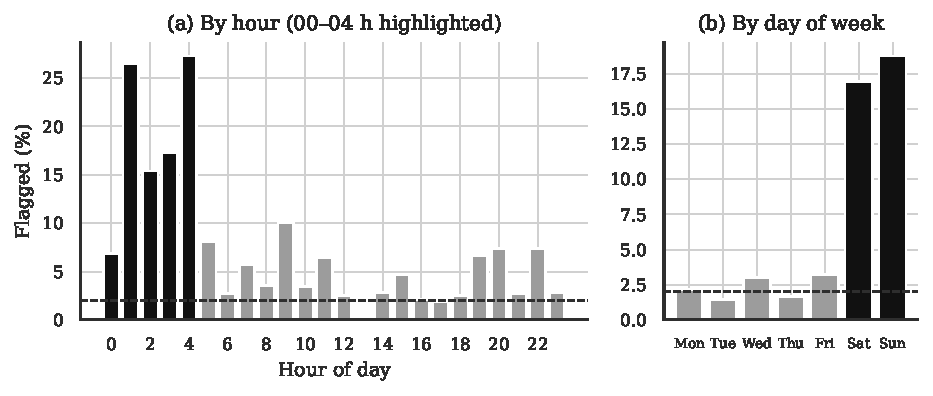
\includegraphics[width=0.85\textwidth]{figures/fig10_temporal.pdf}
\caption{Share of flagged transactions by (a) hour of day and (b) day of week over the full dataset. Dark bars mark the early-morning hours and the weekend; the dashed line is the 2\% target.}
\label{fig:temporal}
\end{figure*}

\subsection{Feature Importance and Interpretability}
\label{sec:res_shap}

Fig.~\ref{fig:shap} shows the 15 features with the largest mean absolute SHAP value. The most influential are \texttt{Month} (0.147), \texttt{USState\_Texas} (0.143), \texttt{TransactionType\_Debit} (0.130), \texttt{Amount\_Dev\_Account} (0.113), and \texttt{USState\_California} (0.113), followed by three occupation indicators (0.083--0.091), the state frequency (0.083), and \texttt{USState\_Arizona} (0.081). The importance spans five categories (temporal, geographic, transaction type, account-relative amount, and demographic), and the largest value is only 0.147, with the fifteenth still at 0.059: no single variable dominates.

\begin{figure}[!t]
\centering
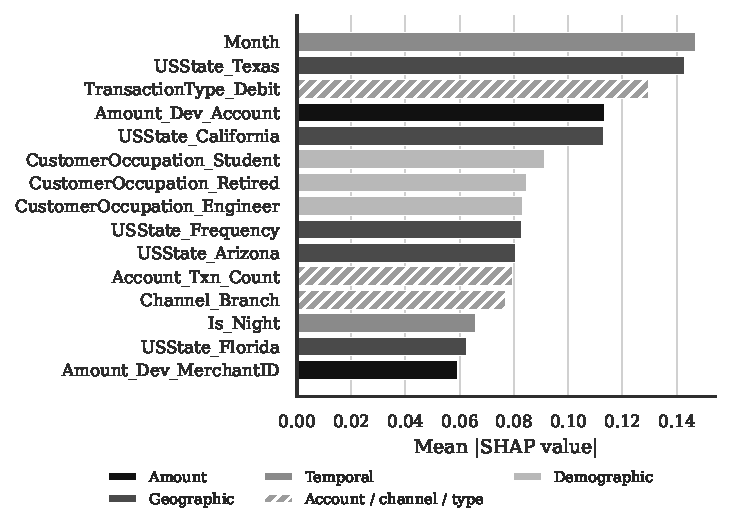
\includegraphics[width=\columnwidth]{figures/fig09_shap.pdf}
\caption{Top 15 features by mean absolute SHAP value, shaded by category. Importance is spread across temporal, geographic, transaction-type, amount, and demographic features.}
\label{fig:shap}
\end{figure}

SHAP importance and the behavioral gaps answer different questions. The gaps describe what separates the few flagged transactions from the rest, while SHAP measures what moves the score of \emph{every} transaction. One-hot indicators of the largest states (Texas, California, and Arizona, with 346, 357, and 183 transactions) and of the debit type (77\% of records) carry large SHAP values because belonging to a common category lowers the score of most transactions, not because they mark anomalies. \texttt{Month} is the most important feature: since the training window ends in early October, the test months lie at or beyond the edge of the range seen in training, which is consistent with the drift reported above. This is a plausible mechanism, not a tested one.

\subsection{Heuristic Sanity Check}

The model was also compared with a transparent hand-built rule that scores high amount, many login attempts, unusual hour, and extreme session duration. On the test window, the Spearman correlation between the two scores is 0.473, and 9.1\% of the top-flagged transactions overlap. The moderate positive correlation indicates that the model is not arbitrary with respect to basic intuition, while the low overlap indicates that it captures more than these four rules. This check is \emph{not} ground truth and is not a second validation of the same kind as the analyses above.

\subsection{Geographic Analysis}

All 52 states in the data were reconciled with the GeoJSON file (0 unmatched), and on the full dataset every state clears the 15-transaction floor, so the map (Fig.~\ref{fig:state_map}) has support everywhere it shows a value. The highest rates are found in Connecticut (16.7\%, 6 of 36), Alaska and West Virginia (15.0\%, 3 of 20 each), Kansas (13.8\%, 4 of 29), and Minnesota (10.5\%, 6 of 57), as listed in Table~\ref{tab:states}. The largest states lie close to the target: Texas at 2.9\% (10 of 346) and California at 2.8\% (10 of 357), while 11 states have no flagged transaction at all.

\begin{figure*}[!t]
\centering
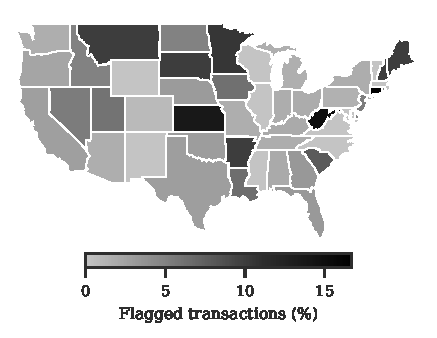
\includegraphics[width=0.85\textwidth]{figures/fig11_state_map.pdf}
\caption{Share of flagged transactions per state on the full dataset (static version of the interactive map). Darker states have higher rates. Every darkest state is covered only by synthetic rows (compare with Fig.~\ref{fig:dataset_map}).}
\label{fig:state_map}
\end{figure*}

\begin{table}[!t]
\renewcommand{\arraystretch}{1.2}
\caption{States with the Highest Anomaly Rate (Full Dataset)}
\label{tab:states}
\centering
\begin{tabular}{lrrrc}
\hline
\textbf{State} & \textbf{$n$} & \textbf{Flag.} & \textbf{Rate} & \textbf{Rows} \\
\hline
Connecticut   & 36 & 6 & 16.67\% & Synthetic \\
Alaska        & 20 & 3 & 15.00\% & Synthetic \\
West Virginia & 20 & 3 & 15.00\% & Synthetic \\
Kansas        & 29 & 4 & 13.79\% & Synthetic \\
Minnesota     & 57 & 6 & 10.53\% & Synthetic \\
\hline
Texas         & 346 & 10 & 2.89\% & Real \\
California    & 357 & 10 & 2.80\% & Real \\
\hline
\end{tabular}
\end{table}

Two facts show that this pattern cannot be read as geographic risk. First, the rate falls with the number of transactions in a state (Spearman $\rho=-0.39$, $p=0.004$ over the 52 states; Fig.~\ref{fig:state_support}): the 20 states with at most 40 transactions are flagged at 7.9\% on aggregate, whereas the 7 states with at least 100 are flagged at 2.2\%. Small denominators produce extreme rates, as in Connecticut, whose 16.7\% rests on six transactions. Second, \emph{all twelve} states with the highest rates are covered only by synthetic rows. Taken together, synthetic states are flagged at 7.3\% and real ones at 2.0\%, so the geographic contrast in the map largely reflects the augmentation described in Section~\ref{sec:augmentation} rather than any regional behavior. A second cut restricted to the stable anomalies of the test window was also computed but is not reported, because only 7 of 51 states reach the support floor on those 560 rows.

\begin{figure}[!t]
\centering
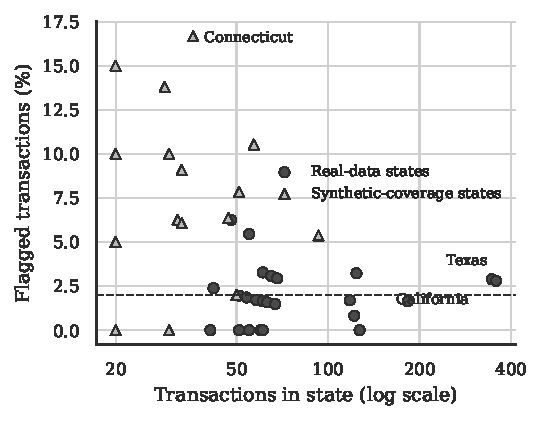
\includegraphics[width=\columnwidth]{figures/fig12_state_support.pdf}
\caption{State anomaly rate versus number of transactions (log scale). The highest rates belong to small states covered only by synthetic rows; large real-data states sit close to the 2\% line.}
\label{fig:state_support}
\end{figure}

% ==========================================================
% 7. DISCUSSION
% ==========================================================

\section{Discussion}

\subsection{Interpretation of the Results}

The results support the general hypothesis: without a single label, the model yields an anomaly ranking that is reproducible, a set of flagged transactions with a clear behavioral signature, and limitations that can be measured rather than assumed. Each analysis also explains part of the others. The stability analysis shows that the \emph{score} is the reliable output and the \emph{flag} is the fragile one, because flags depend on where a threshold cuts a continuous ranking. The temporal analysis shows that this threshold is also the component that degrades over time. Together, they suggest that, in an operational setting, transactions should be prioritized by score, and the cutoff should be treated as an adjustable review budget rather than as a property of the model.

\textit{Temporal drift.} The monthly view moves the discussion from ``the test window is different'' to ``the score level rises steadily from August.'' Without labels, it is impossible to tell whether this reflects changing customer behavior, a seasonal effect (the dataset covers a single year, so seasonality cannot be separated from trend), the edge effect of \texttt{Month}, or noise in a small sample. What can be stated is that a fixed, train-derived cutoff over-flags later periods, by a factor of 2.8 in real rows and 3.4 overall.

\textit{Behavioral interpretation.} The behavioral contrast is the most intuitive result: flagged transactions are large, and large \emph{for their context}. This agrees with what an analyst would examine first, and with the moderate correlation to the hand-built rule. Weekend and early-morning timing are the strongest secondary signals, but both are rare slots, so they mainly indicate what Isolation Forest considers unusual, which is not necessarily what is risky.

\textit{Geographic patterns.} The map does what it was designed to do, namely show every state, but the audit shows that its most striking colors come from small samples and from synthetic rows. This is an important methodological lesson: data added for presentation purposes is not neutral once it passes through the model.

\subsection{Hypothesis Evaluation}
\label{sec:hypothesis_eval}

Table~\ref{tab:hypotheses} summarizes the evidence for each hypothesis.

\begin{table*}[!t]
\renewcommand{\arraystretch}{1.25}
\caption{Evaluation of the Hypotheses}
\label{tab:hypotheses}
\centering
\begin{tabular}{p{0.20\textwidth}p{0.55\textwidth}p{0.15\textwidth}}
\hline
\textbf{Hypothesis} & \textbf{Evidence} & \textbf{Outcome} \\
\hline
H1: ranking more stable than flag & Spearman 0.899 vs. Jaccard 0.689 (non-overlapping distributions); bimodal per-transaction stability: 21 borderline vs. 16 always flagged & Supported \\
H2: fixed threshold does not transfer & 2.02\% $\rightarrow$ 2.32\% $\rightarrow$ 6.79\%; 4.64--6.79\% across seeds; real rows only: 1.5\% $\rightarrow$ 4.2\%; drift starts in August & Supported \\
H3: amount-driven differences & Top five gaps are amount features (1.83--1.94); weekend is the largest non-amount gap (1.29) & Supported \\
H4: multifactorial anomaly & Five feature categories in the SHAP top 15; maximum importance 0.147 & Supported \\
H5: geography is descriptive & Rate vs. support $\rho=-0.39$; top 12 states are synthetic; 7.3\% synthetic vs. 2.0\% real & Supported, with an added confound \\
\hline
\end{tabular}
\end{table*}

H3 and H4 may appear to be in tension, since amount dominates the contrast but not SHAP. As explained in Section~\ref{sec:res_shap}, they measure different things: the contrast describes the extreme tail, whereas SHAP describes the score of the whole population. H5 is supported more strongly than anticipated, because, in addition to the expected sample-size effect, the synthetic rows act as a confounder that was not part of the original hypothesis.

\subsection{Implications of Using Unsupervised Anomaly Detection}

The framework shows that useful, falsifiable statements can be made about an unlabeled model: stability, temporal transfer, behavioral coherence, and geographic support can all be checked without any fraud label. In return, the framework cannot measure whether flagged transactions are fraudulent. Its natural role is therefore to \emph{prioritize} cases for human review, as a first filter whose output is checked by analysts and, eventually, converted into the labels that a supervised model would require.

% ==========================================================
% 8. LIMITATIONS
% ==========================================================

\section{Limitations}

\begin{enumerate}
    \item \textit{No ground-truth fraud labels.} Every result is a statement about statistical unusualness relative to the training distribution, never about confirmed fraud, and supervised metrics cannot be computed.
    \item \textit{Anomalies cannot be interpreted as confirmed fraud.} Rare but legitimate behavior, such as weekend or early-morning transactions, is flagged for being rare.
    \item \textit{Temporal distribution shift.} A single train-derived cutoff over-flags later periods by a factor of 2.8--3.4. With only one year of data, drift and seasonality cannot be separated, and the 60-day test window is short.
    \item \textit{Sensitivity of binary thresholding.} Jaccard alone (0.689) would understate the consistency of the model; the instability concentrates at the cutoff, not in the ranking.
    \item \textit{Synthetic rows.} 781 of the 3,293 rows (23.7\%) are synthetic and were added for map coverage. They are flagged 3.6 times more often than real rows and they influence the model, the feature statistics, and especially the geographic results.
    \item \textit{Geographic support limitations.} Many states have only 20--40 transactions, and only 7 of 51 states reach the support floor in the test window, so no state-level robustness claim can be made.
    \item \textit{Dataset-specific findings.} The dataset is small (560 test transactions), and the gaps and importances should be read as descriptive, not as precise estimates.
    \item \textit{Need for external validation.} The heuristic comparison is only a sanity check; validating the framework requires labeled data, analyst feedback, or a second dataset.
\end{enumerate}

% ==========================================================
% 8b. REPRODUCIBILITY  (new section)
% ==========================================================

\section{Reproducibility}

All results come from a single, versioned pipeline. Training and artifact generation are run with \texttt{python -m scripts.train\_pipeline}, and the figures in this paper with \texttt{python -m paper.make\_figures}, which re-runs the unchanged model (seed 42) and checks that its threshold matches the stored artifacts. The dataset augmentation is reproduced with \texttt{python -m scripts.augment\_dataset} (seed 42). The model configuration (300 trees, contamination 0.02) was fixed before the analysis and was not modified in response to any result reported here.

% ==========================================================
% 9. CONCLUSION
% ==========================================================

\section{Conclusion}

This work reformulated financial fraud detection as an unsupervised anomaly detection problem, motivated by the absence of fraud labels in the available data. An Isolation Forest trained with a strictly temporal split was used to score 3,293 US bank transactions, and its output was examined from five complementary angles: temporal transfer, stability, behavioral contrast, feature attribution, and geography.

The main findings are as follows. First, the anomaly ranking is stable across seeds ($\rho=0.899$), while the binary flag is less so (Jaccard $=0.689$), and 16 test transactions form a core flagged under every seed. Second, a threshold fixed on training data does not keep its 2\% rate: it flags 6.79\% of the test window, and the monthly view shows a progressive drift that begins in August and is present even in real transactions alone. Third, flagged transactions are distinguished mainly by amount, both absolute and relative to hour, state, merchant, and balance, while the model's overall notion of anomaly is multifactorial. Fourth, the geographic pattern on the US map is explained by sample size and by the synthetic coverage rows, and must be read descriptively.

The framework thus makes it possible to identify unusual transactions, quantify how much each flag can be trusted, detect when a threshold stops being valid, and explain what makes a transaction unusual, all without labeled data. Future work includes recalibrating the threshold on a rolling window and monitoring drift explicitly, rerunning the analysis on real transactions only and on multi-year data to separate drift from seasonality, comparing Isolation Forest with other detectors such as LOF and autoencoders, and incorporating analyst feedback to turn the most stable anomalies into the first labels of a semi-supervised model.

%  ==========================================================
% ACKNOWLEDGMENT
% ==========================================================

\section*{Acknowledgment}

The authors thank ITESO, Universidad Jesuita de Guadalajara, for providing the academic environment and resources that supported this research.

% ==========================================================
% REFERENCES
% ==========================================================

\printbibliography

% ==========================================================
% APPENDIX  (new)
% ==========================================================

\appendices

\section{Score Versus Stability}

\begin{figure}[H]
\centering
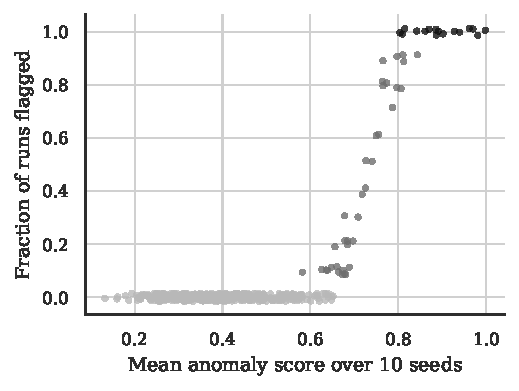
\includegraphics[width=\columnwidth]{figures/figA1_score_vs_stability.pdf}
\caption{Mean anomaly score over the ten seeds versus the fraction of runs in which each test transaction is flagged (small vertical jitter added). Transactions flagged in every run (darkest) all have mean scores above 0.80; partially flagged ones (mid gray) lie around the per-seed thresholds, confirming that flag instability is concentrated near the cutoff.}
\label{fig:score_vs_stab}
\end{figure}

\end{document}
